% Optional include file for the final KBS figure set.
%
% The manuscript includes its figures directly from `sections/6_experiments.tex`
% and `sections/3_problem.tex`. This file mirrors the same six figures for
% tooling that builds the figure list from a single place; keep it in sync with
% `SOURCES.md` when a figure changes.
%
% Figure numbering follows order of appearance:
%   Fig. 1 fig1_conceptual, Fig. 2 fig2_headroom, Fig. 3 fig3_multitarget_delta,
%   Fig. 4 fig3_scaling, Fig. 5 fig5_real_observability, Fig. 6 fig4_frontier.

\begin{figure}[tbp]
  \centering
  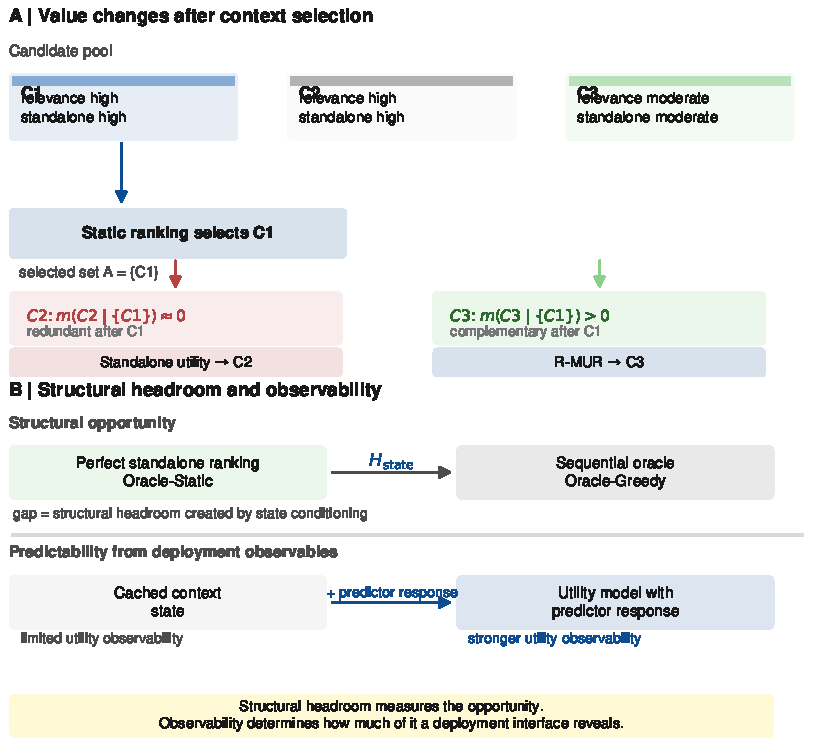
\includegraphics[width=0.98\linewidth]{figures/fig1_conceptual.pdf}
  \caption{State-conditioned context selection. A candidate's standalone value
  can change after similar information is selected. The gap between a
  standalone oracle and a sequential oracle measures structural headroom,
  while the information available at inference time determines how much of
  that value a router can estimate.}
  \label{fig:conceptual}
\end{figure}

\begin{figure}[tbp]
  \centering
  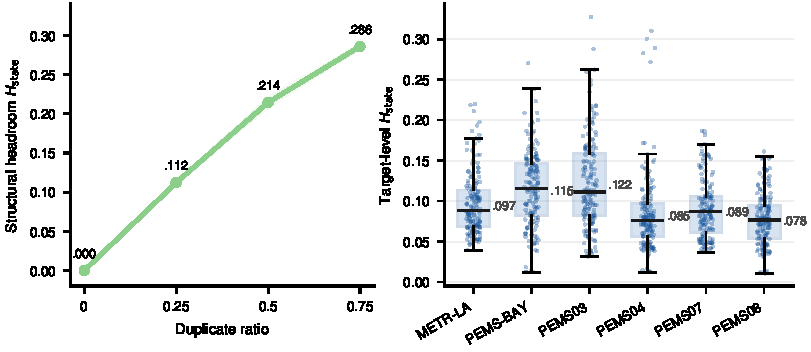
\includegraphics[width=0.98\linewidth]{figures/fig2_headroom.pdf}
  \caption{Redundancy creates state-conditioning headroom. The gap between
  Standalone Utility and the sequential oracle grows with the duplicate ratio,
  and R-MUR recovers part of that gap.}
  \label{fig:headroom}
\end{figure}

\begin{figure}[tbp]
  \centering
  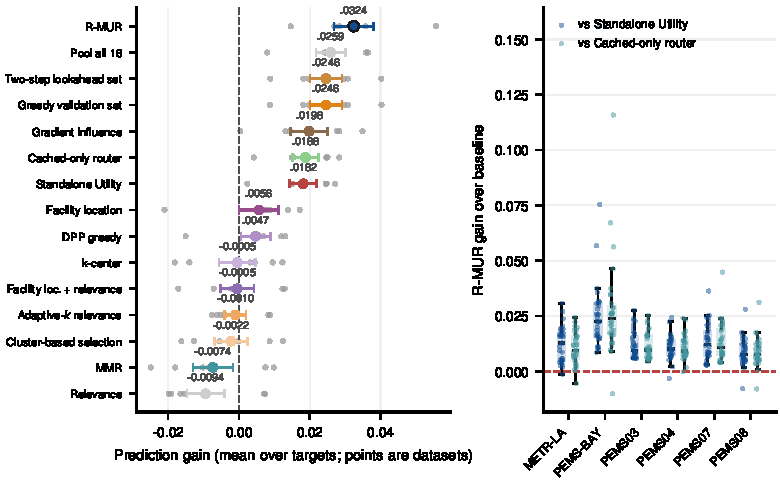
\includegraphics[width=0.98\linewidth]{figures/fig3_multitarget_delta.pdf}
  \caption{Multi-target routing results. Left: prediction gain of deployable
  methods on the six benchmarks. Right: distribution over targets of the R-MUR
  gain over Standalone Utility and over the cached-only router.}
  \label{fig:target-delta}
\end{figure}

\begin{figure}[tbp]
  \centering
  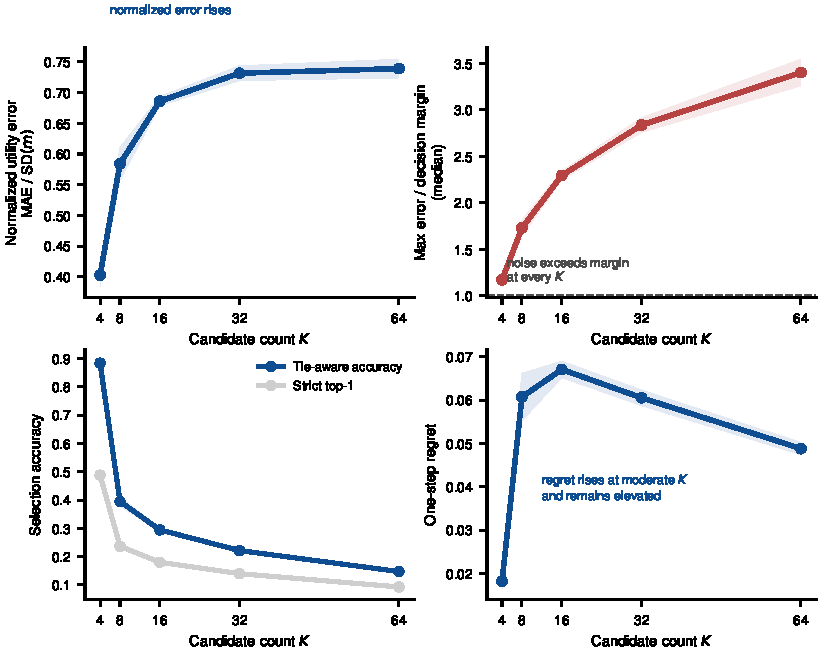
\includegraphics[width=0.98\linewidth]{figures/fig3_scaling.pdf}
  \caption{Candidate-set growth creates a ranking bottleneck. Pointwise utility
  error improves in absolute terms while the decision margin shrinks, so
  selection accuracy falls and one-step regret rises.}
  \label{fig:scaling}
\end{figure}

\begin{figure}[tbp]
  \centering
  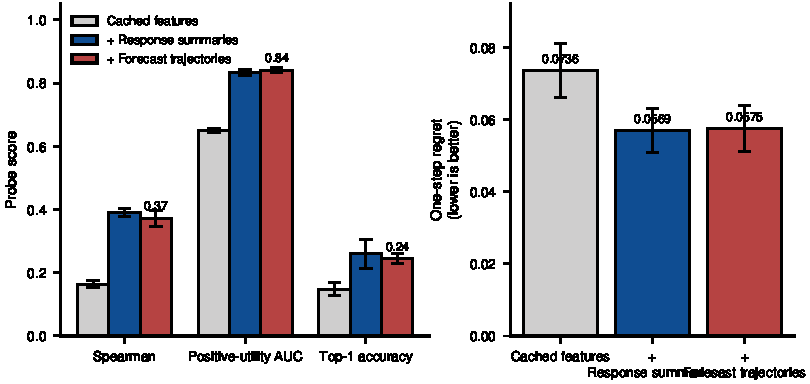
\includegraphics[width=0.98\linewidth]{figures/fig5_real_observability.pdf}
  \caption{Utility predictability. Compact summaries of the predictor response
  improve rank correlation, positive-utility AUC, and top-1 accuracy over
  cached context features, and they lower one-step regret.}
  \label{fig:observability}
\end{figure}

\begin{figure}[tbp]
  \centering
  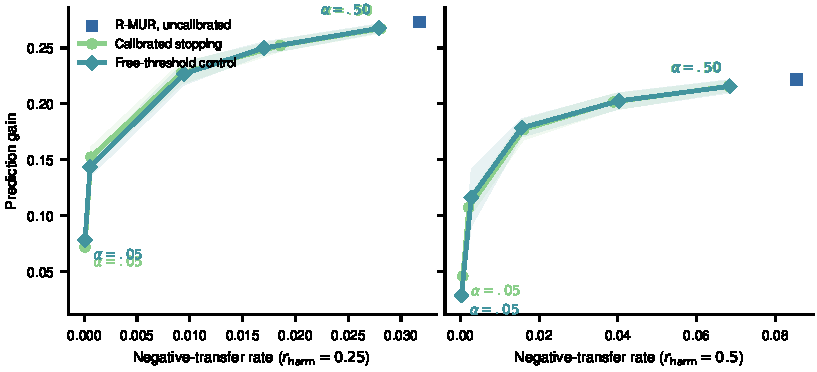
\includegraphics[width=0.98\linewidth]{figures/fig4_frontier.pdf}
  \caption{Calibrated stopping traces a gain--harm frontier at two harmful
  candidate fractions. Raising the calibration level increases both gain and
  negative-transfer rate; at the highest level the calibrated policy nearly
  matches the gain of the uncalibrated router while reducing harm.}
  \label{fig:frontier}
\end{figure}
